\documentclass[Shakespeare.tex]{subfiles}

\newpage
\begin{document}

\section{Shakespeare Application}

The Shakespeare application allows users to browse through a Shakespearean play and analyze its content, read some specific parts and maybe find related information. The application was written in the eXist IDE environment and all the code can be found on GitHub link from section 1. Figure \ref{fig:shakespearemain} shows a screenshot of the homepage for the application with the available plays listed in alphabetical order.

\begin{figure} [H]
	\centering
	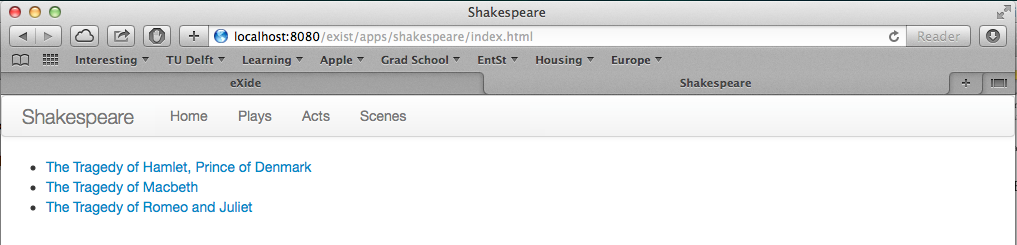
\includegraphics[width=1\textwidth]{./Figures/ShakespeareMain.png}
	\caption{Shakespeare Application}
	\label{fig:shakespearemain}
\end{figure}

\subsection{Architecture}
The architecture for the Shakespeare is detailed below:

\begin{enumerate}
	\item Navigation panel - Allows user to browse between plays, acts, scenes and characters
	\item Contents - When a play is selected, the contents pages shows the acts, scenes and characters involved in the play
		\begin{enumerate}
			\item Act - Shows the entire act of the play
			\item Scene - Shows the entire scene from the act of the selected play with characters involved in that scene shown at the top of the page.
			\item Character - Shows every act/scene where the character speaks
			\begin{enumerate}
				\item Selecting a specific scene/act where the character has lines opens up a drop-down panel that shows all of the character's lines from that act/scene
			\end{enumerate}
		\end{enumerate}	
	\item Scene/Act - Character links present in the layout show all the lines of that character from all scenes/acts
\end{enumerate}

XQUERY and XSLT was used to build the interface for the Shakespeare application and the software was written in the eXist environment. As a starting point, we used the XSLT templates from the Shakespeare application and modified the code to fit our application's needs. We added 2 additional XSLT files for our application's styling and these were also built upon existing demo examples in the eXist application folder. The plays (Hamlet, Macbeth, Romeo and Juliet) were added to the application as collections. The entire source code can be found at the GitHub link from Section 1. Additional styling was done using the bootstrap CSS and jQuery stylesheets already available within the shared folder in eXist.

Figure \ref{fig:macbethtoc} below shows the table of contents for Macbeth. The acts, scenes and characters are listed.
\begin{figure} [H]
	\centering
	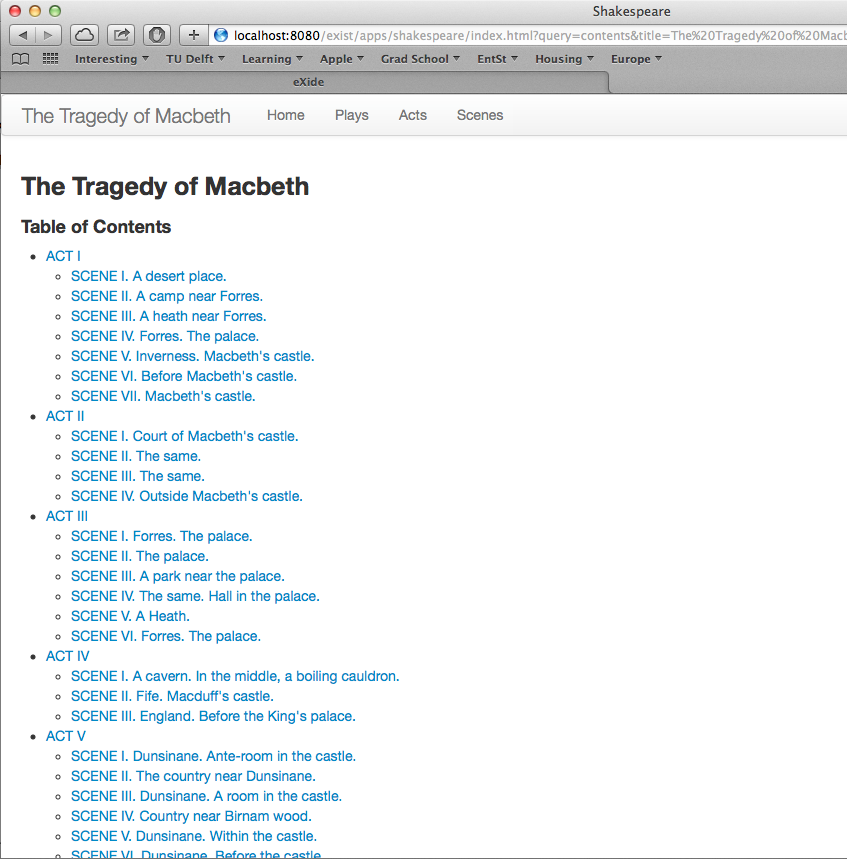
\includegraphics[width=1\textwidth]{./Figures/MacbethTOC.png}
	\caption{Macbeth Contents Page}
	\label{fig:macbethtoc}
\end{figure}

\subsection{Character Lines Display}
Figure \ref{fig:macbethlines} shows Macbeth's lines from Act V, Scene VIII in a drop-down panel box. The navigation panel at the top of the page is always accessible to the user and they can always jump between scenes, acts and/or characters once a play is selected.

\begin{figure} [H]
	\centering
	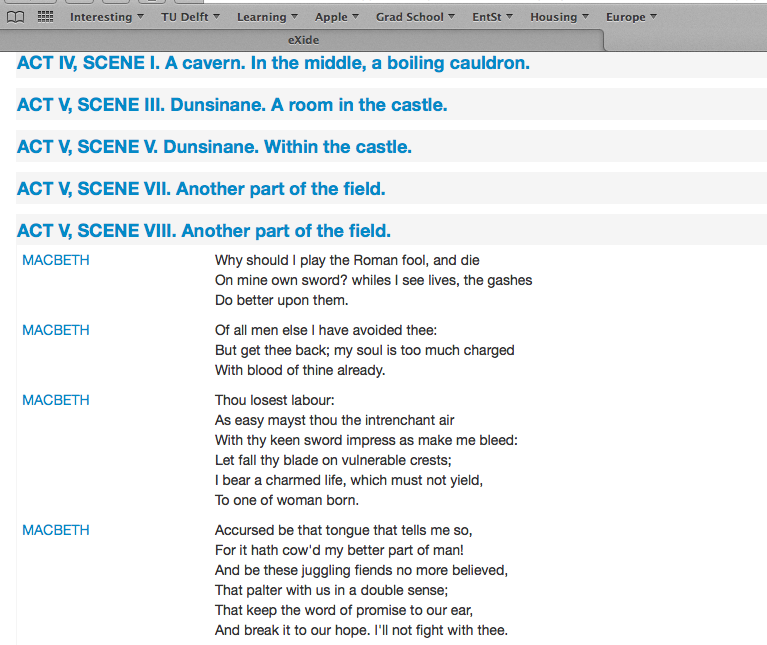
\includegraphics[width=1\textwidth]{./Figures/MacbethCharacterSceneDetails.png}
	\caption{Macbeth's lines from Act V, Scene VIII}
	\label{fig:macbethlines}
\end{figure}

\end{document}